% !TEX root = ../Ausarbeitung.tex
\section{Problems}\label{sec:problems}
While working on the challenge, some problems arose with the neurorobotics platform itself as well as the server infrastructure around it.
The simulations in the neurorobotics platform are non-deterministic which leads to non-reproducible results.
This non-determinism probably results from floating point inaccuracy.
In addition to that, the grasping of the cylinder is very unreliable.
If the cylinder is grasped too tightly the robot starts shaking, sometimes resulting in the hand exploding and the cylinder flying huge distances (see \autoref{fig:dispersed}).
In some extreme cases, the whole table the robot is mounted to moves, which results in the grasping not working afterwards due to a change in the relation of the robot and world coordinate systems.
There were also problems with the platform crashing regularly because of different reasons.
All these problems occurred on the server install of the platform.
In absence of a working local install, it wasn't possible to check if they were specific to the server install or the platform itself.

\begin{figure}[h]
\centering
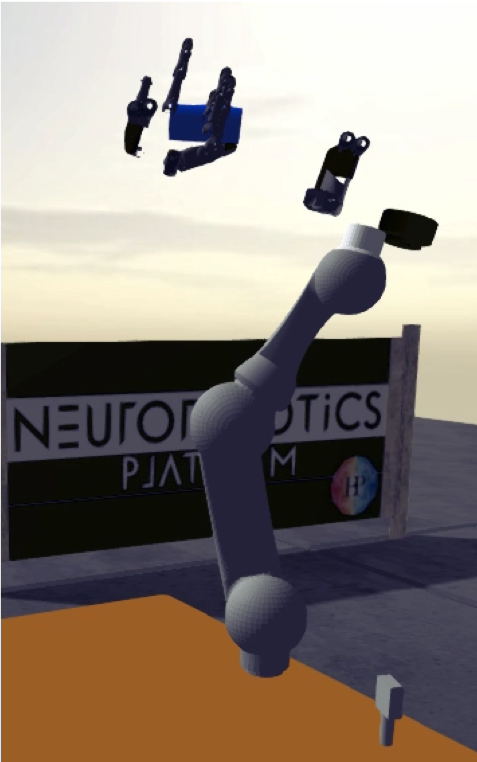
\includegraphics[width=.95\columnwidth]{figures/dispersed_robot.png}
\caption{Occasionally, different parts of the robot scatter.}
\label{fig:dispersed}
\end{figure}